\chapter{複合系、エンタングルメント、一重項}

\lectureoverview{光子放出に関する問いは、量子的事象とその集団平均との違いを明らかにする。その区別は自然に測定、収縮、そして系を装置とともに扱う必要性へと導く。そこで我々は二つの系のテンソル積状態空間を構成し、二つのスピンに特殊化し、積状態とエンタングル状態を区別し、各一スピン可観測量を複合空間に埋め込む。そして一重項状態が決定的な例を与える。各スピンは局所的に偏極していないが、等しい成分は完全に反相関している。その基底に依らない形は、ベル定理および非古典的相関と超光速シグナリングとの区別への準備となる。}

\section{重ね合わされたスピンからの離散的遷移}

\(z\)軸に沿った磁場中の一つのスピンから始める。\(\hbar=1\)とする単位系では、
\begin{equation}
H=\frac{\omega}{2}\sigma_z,
\qquad
E_+=+\frac{\omega}{2},
\qquad
E_-=-\frac{\omega}{2}.
\label{eq:l6-spin-hamiltonian}
\end{equation}
二つの準位は次で隔てられている。
\begin{equation}
\Delta E=E_+-E_-=\omega.
\label{eq:l6-energy-gap}
\end{equation}
放射場を含めると、上準位にあるスピンは下準位へ落ちてエネルギー\(\omega\)の光子を放出しうる。すでに下準位にあるスピンには、放射できるより低いスピン状態が存在しない。

\begin{figure}[htbp]
\centering
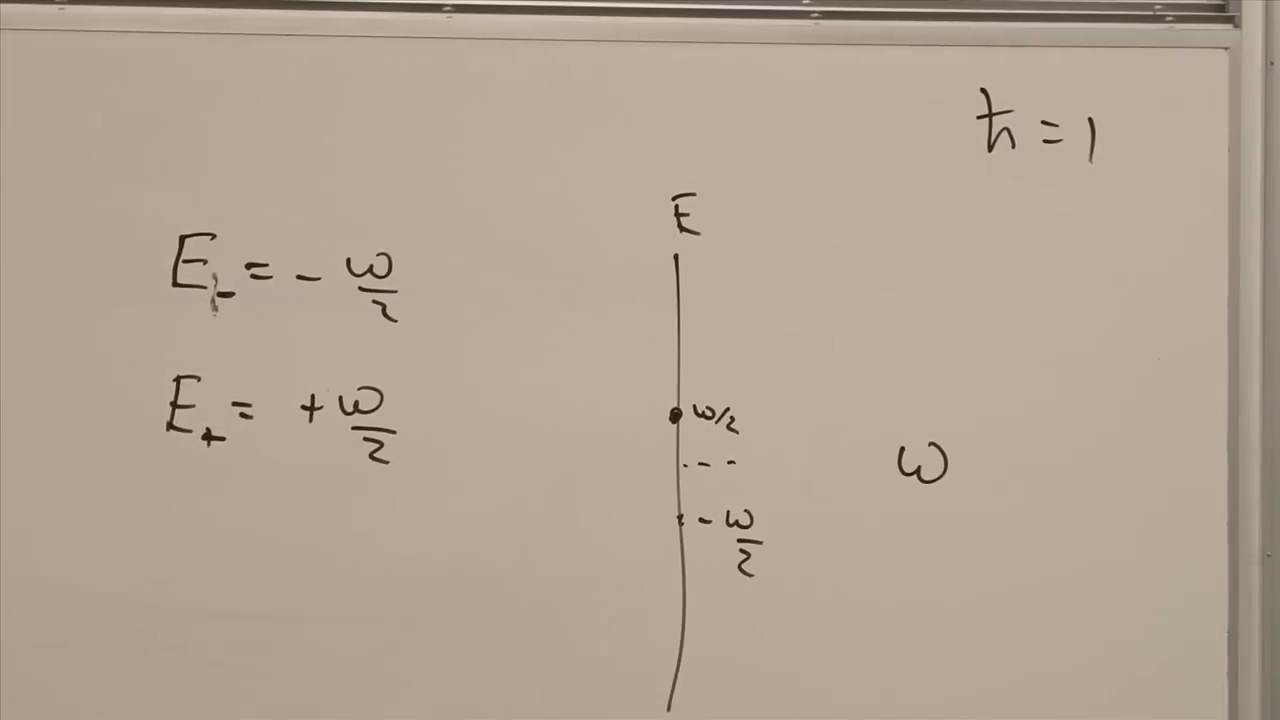
\includegraphics[width=0.86\textwidth]{lecture_06_figure_01.png}
\caption{二つのスピンエネルギー準位とその間隔\(\omega\)。ただし\(\hbar=1\)とする。}
\lectureframe{00:02:35}
\end{figure}

微妙な場合は横向きに準備されたスピンである。古典的な磁気回転子は、磁場とのなす角の余弦に比例して連続的に変化するエネルギーをもつ。それは角振動数\(\omega\)で歳差運動し、同じ振動数で放射し、徐々に最小エネルギーの向きへ落ちていく。全放射エネルギーは初期角度に連続的に依存する。最初に水平な回転子は、頂点から始まる回転子の半分のエネルギーを放出する。

量子力学はその古典的答えを平均としてのみ保つ。
\begin{equation}
\ket{\psi}=\alpha\ket{u}+\beta\ket{d},
\qquad
|\alpha|^2+|\beta|^2=1,
\label{eq:l6-superposed-spin}
\end{equation}
と書く。ここで\(\ket{u}\)と\(\ket{d}\)は上準位と下準位のエネルギー固有状態である。上成分は崩壊しうるが、下成分は崩壊できない。したがって
\begin{equation}
P(\text{one photon})=|\alpha|^2,
\qquad
P(\text{no photon})=|\beta|^2.
\end{equation}
光子が放出されるならば、そのエネルギーは準位間隔\(\omega\)の全体であり、その一部ではない。それでも平均放出エネルギーは
\begin{equation}
\expect{E_{\rm emitted}}=|\alpha|^2\omega.
\end{equation}
である。\(x\)に沿ったスピンでは\(|\alpha|^2=|\beta|^2=1/2\)なので、平均は\(\omega/2\)である。個々の事象は依然として、エネルギー\(\omega\)の光子を一つ放出するか、光子を放出しないかのいずれかである。連続的な古典的結果は集団平均に属し、離散性は各事象に属する。

\begin{classroomqa}
\audiencequestion{吸収される光子は準位間隔にどれほど正確に一致しなければならないか。}
\lecturerresponse{共鳴は有限の線幅をもつ。励起状態の寿命が\(\tau\)ならば、その特徴的エネルギー幅は\(\Delta E\sim\hbar/\tau\)の程度である。一般に磁気双極子モーメントが大きいほど放射場との結合が強くなり、寿命を短くし、線を広げる。これは不安定な準位に関係する形でのエネルギー・時間不確定性関係である。}
\end{classroomqa}

\begin{classroomqa}
\audiencequestion{光子放出それ自体がスピンを測定する装置として働きうるか。}
\lecturerresponse{それは崩壊が起こったかどうかを明らかにしうるが、ここで必要な理想的な繰り返し可能測定の模型ではない。スピン成分の測定は、記録された値に対応する固有状態にスピンを残すべきである。それに対して崩壊は、放出されたすべての分岐を下準位へ駆り立てるので、可能な二つの入力値の両方を、それぞれに対応する固有状態を保ちながら単に記録するものではない。}
\end{classroomqa}

\section{収縮と複合系の必要性}

介入と介入の間では、孤立した状態はSchr\"odinger方程式に従って発展する。測定は通常、追加の規則として述べられる。\(L\)が正規直交固有ベクトル\(\ket{\lambda_i}\)をもつとし、
\begin{equation}
\ket{\psi}=\sum_i\alpha_i\ket{\lambda_i},
\qquad
L\ket{\lambda_i}=\lambda_i\ket{\lambda_i}.
\label{eq:l6-measurement-expansion}
\end{equation}
と展開する。測定は確率\(|\alpha_k|^2\)で一つの値\(\lambda_k\)を与え、その後状態は
\begin{equation}
\ket{\psi}\longrightarrow\ket{\lambda_k}.
\label{eq:l6-collapse}
\end{equation}
となる。測定後の記述から他の成分が消えることを収縮と呼ぶ。

\begin{figure}[htbp]
\centering
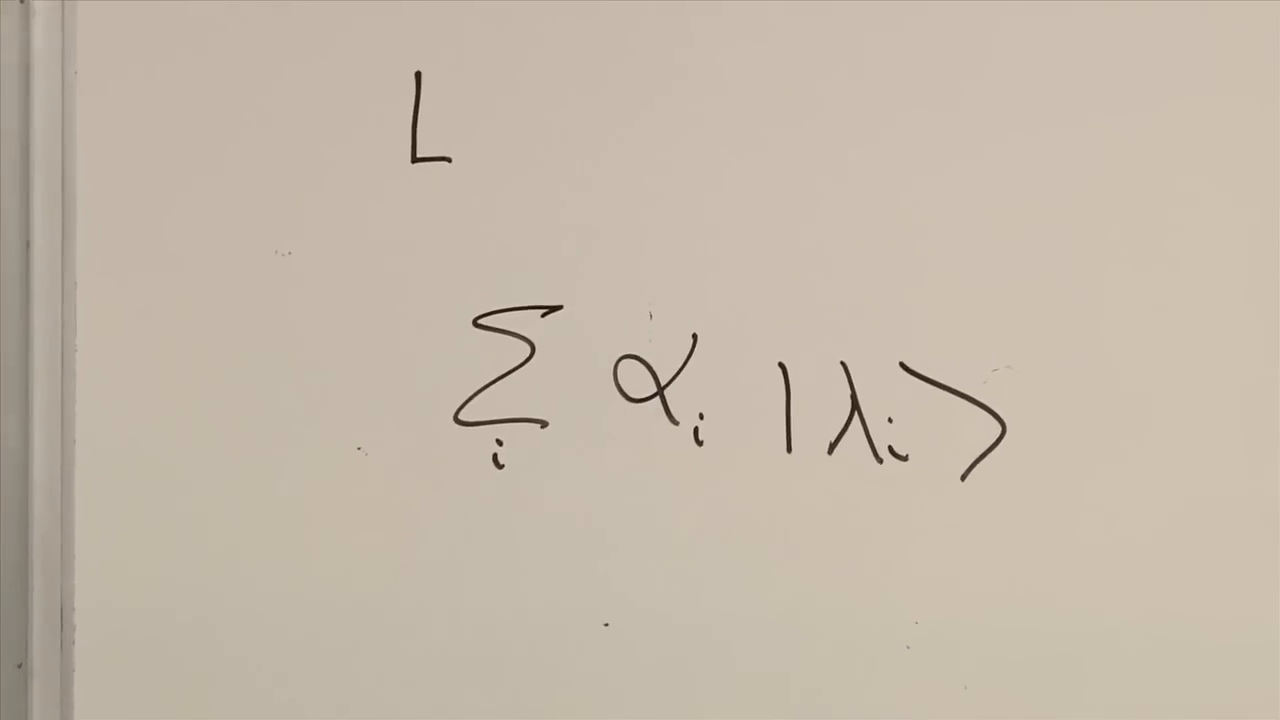
\includegraphics[width=0.84\textwidth]{lecture_06_figure_02.png}
\caption{可観測量\(L\)の固有基底で展開された状態。一つの結果が選ばれる前のものである。}
\lectureframe{00:12:35}
\end{figure}

\begin{classroomqa}
\audiencequestion{収縮規則の何が問題なのか。}
\lecturerresponse{測定結果を予測するための操作的規則としては何も問題はない。概念的緊張は、装置それ自体が物理系であるということである。対象と装置の両方が量子力学に従うならば、なぜそれらの相互作用はユニタリなSchr\"odinger発展に加えて第二の力学法則を必要とするのか。ここで取る道は、対象と装置を一つのより大きな量子系として記述することである。}
\end{classroomqa}

鋭い系と装置の境界は、歴史的論争の中心点であった。その論争を宣言によって決着させるのではなく、まず量子系がどのように組み合わされるかを学ぶ。合成状態空間が利用可能になれば、測定は系と装置を相関させる相互作用として研究できる。したがって当面の数学的問いは次のとおりである：
\begin{quote}
二つの量子系が与えられたとき、全体の状態空間は何か？
\end{quote}

\section{テンソル積状態空間}

系を\(A\)および\(I\)と呼び、そのヒルベルト空間を\(\mathcal S_A\)および\(\mathcal S_I\)とする。それらの合成空間は
\begin{equation}
\mathcal S_{AI}=\mathcal S_A\otimes\mathcal S_I.
\label{eq:l6-tensor-space}
\end{equation}
である。二つの因子に対して正規直交基底\(\{\ket{a}\}\)および\(\{\ket{i}\}\)を選ぶ。第一の系の各基底ベクトルを第二の系の各基底ベクトルと対にする：
\begin{equation}
\ket{a}\otimes\ket{i}\equiv\ket{a\,i}.
\end{equation}
因子空間の次元が\(D_A\)および\(D_I\)ならば、
\begin{equation}
\dim\mathcal S_{AI}=D_A D_I.
\end{equation}
である。内積は因数分解し、
\begin{equation}
\braket{b\,j}{a\,i}
=\braket{b}{a}\braket{j}{i}
=\delta_{ba}\delta_{ji}.
\label{eq:l6-tensor-inner-product}
\end{equation}
となる。したがって、いずれかの部分系のラベルが異なれば、二つの合成基底状態は直交する。

\begin{figure}[htbp]
\centering
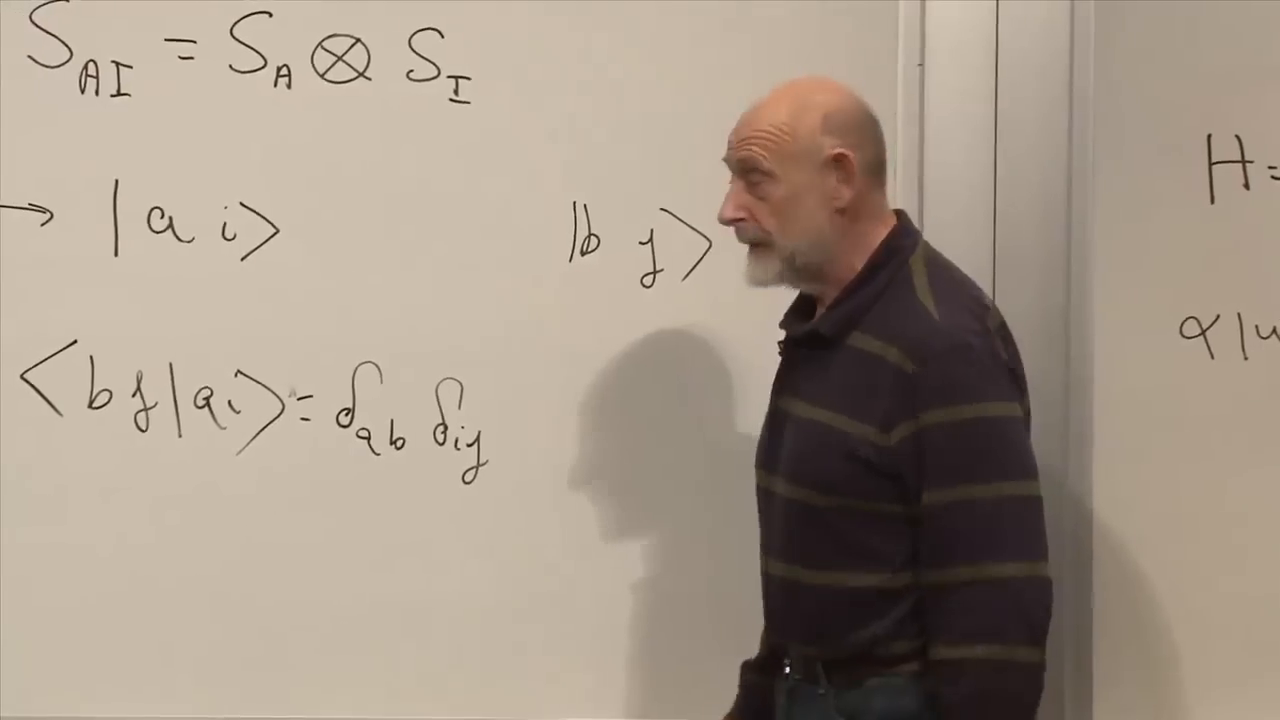
\includegraphics[width=0.86\textwidth]{lecture_06_figure_03.png}
\caption{分離した状態空間、そのテンソル積、および対にされた正規直交基底。}
\lectureframe{00:24:05}
\end{figure}

対にされた基底ベクトルは空間全体ではない。それらの完全な線形包は：
\begin{equation}
\ket{\Psi}=\sum_{a,i}c_{ai}\ket{a\,i},
\qquad
\sum_{a,i}|c_{ai}|^2=1.
\label{eq:l6-general-tensor-state}
\end{equation}

\begin{classroomqa}
\audiencequestion{\(\ket{a}\)と\(\ket{i}\)は任意のベクトルか？}
\lecturerresponse{ここではそれらは選ばれた正規直交基底の要素である。どちらの因子でも任意の正規直交基底を用いてよい。それらの基底ベクトルを対にすることにより合成空間の正規直交基底が構成され、その後、任意のベクトルは式~\eqref{eq:l6-general-tensor-state}のように線形結合を取ることによって得られる。}
\end{classroomqa}

\begin{classroomqa}
\audiencequestion{テンソル積は選ばれた基底に依存するか？}
\lecturerresponse{その座標記述は依存するが、空間は依存しない。どちらかの部分系で基底を変えても、\(\mathcal S_A\otimes\mathcal S_I\)内の同じベクトルを記述するために用いられる誘導基底が変わるだけである。}
\end{classroomqa}

\section{二つのスピンと積状態}

次に二つのスピンを取る。第一の成分を\(\sigma_x,\sigma_y,\sigma_z\)、第二の成分を\(\tau_x,\tau_y,\tau_z\)と表す。\(z\)基底では、合成基底は
\begin{equation}
\ket{uu},\qquad \ket{ud},\qquad \ket{du},\qquad \ket{dd}.
\label{eq:l6-two-spin-basis}
\end{equation}
である。第一の位置は常に\(\sigma\)を指し、第二の位置は\(\tau\)を指す。一般の状態は
\begin{equation}
\ket{\Psi}
=c_{uu}\ket{uu}+c_{ud}\ket{ud}
+c_{du}\ket{du}+c_{dd}\ket{dd}.
\label{eq:l6-general-two-spin}
\end{equation}

\begin{classroomqa}
\audiencequestion{二つのスピンが相互作用するなら、基底ベクトル自体は変化するか？}
\lecturerresponse{力学に従うために固定された基底は必要ない。選ばれた基底では、相互作用は係数\(c_{ab}(t)\)を変化させ、\(\ket{uu},\ket{ud},\ket{du},\ket{dd}\)の定義を変化させない。\(\ket{uu}\)として始まる状態は重ね合わせへ、あるいは\(\ket{dd}\)へさえも発展しうるが、座標基底は同じままである。}
\end{classroomqa}

この構成は整合性のテストにも合格しなければならない。スピンが遠く離れており、\(\sigma\)のみを調べるなら、予測は\(\tau\)が導入される前に展開された一スピン理論と一致しなければならない。テンソル積はその局所理論を保持するように設計されている。

いくつかの二スピン状態は独立に準備されたスピンを記述する。例えば、
\begin{equation}
\ket{R}=\frac{\ket{u}+\ket{d}}{\sqrt2}
\end{equation}
を\(x\)成分の\(+1\)固有状態とする。すると
\begin{equation}
\ket{u}_{\sigma}\otimes\ket{R}_{\tau}
=\frac{\ket{uu}+\ket{ud}}{\sqrt2}.
\label{eq:l6-up-right-product}
\end{equation}

\begin{classroomqa}
\audiencequestion{二つの因子を異なる軸に沿って準備してもよいか？}
\lecturerresponse{はい。各因子は任意の一スピン状態でありうる。式~\eqref{eq:l6-up-right-product}では、第一のスピンは\(z\)に沿って確定しており、第二のスピンは\(x\)に沿って確定している。第二の因子を\(z\)基底で展開することは、同じ積状態を合成基底で書き直すだけである。}
\end{classroomqa}

最も一般の積状態は
\begin{align}
\ket{\Psi_{\rm prod}}
&=(\alpha_u\ket{u}+\alpha_d\ket{d})
\otimes(\beta_u\ket{u}+\beta_d\ket{d})\\
&=\alpha_u\beta_u\ket{uu}
+\alpha_u\beta_d\ket{ud}
\\
&\quad
+\alpha_d\beta_u\ket{du}
+\alpha_d\beta_d\ket{dd}.
\label{eq:l6-product-expansion}
\end{align}

\begin{figure}[htbp]
\centering
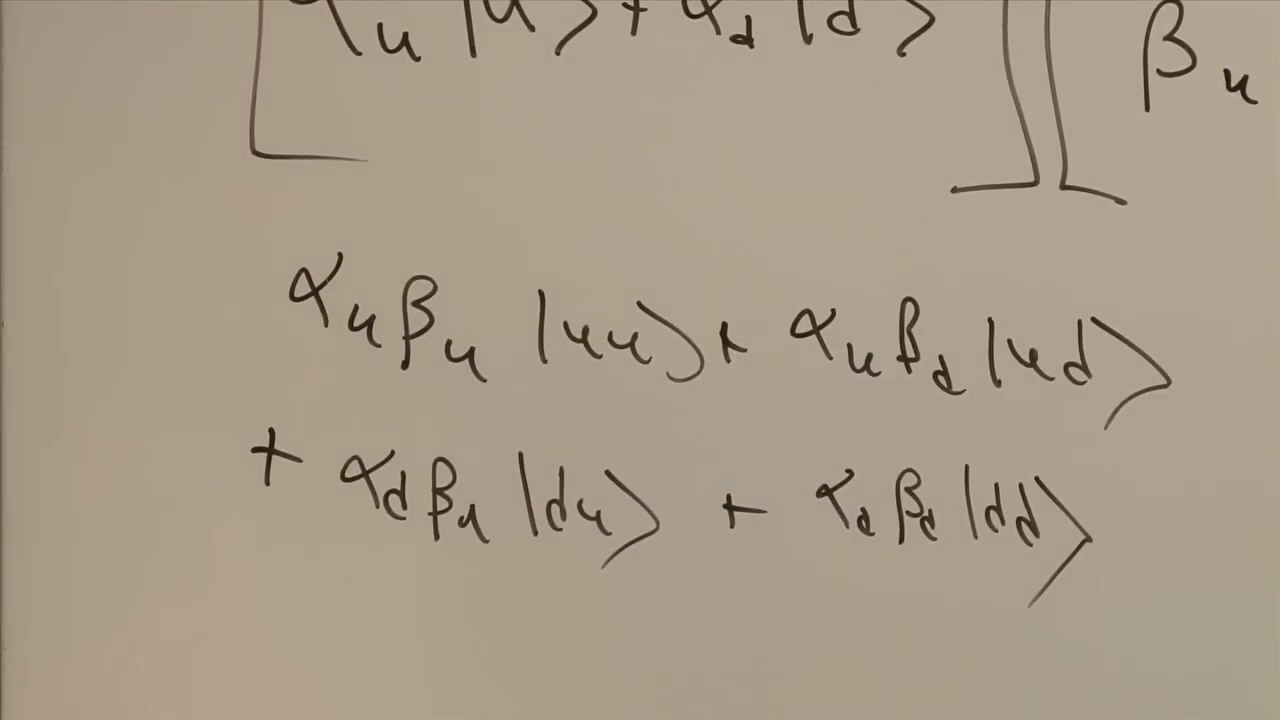
\includegraphics[width=0.86\textwidth]{lecture_06_figure_04.png}
\caption{四状態合成基底で展開された因数分解された二スピン状態。}
\lectureframe{00:37:45}
\end{figure}

\begin{classroomqa}
\audiencequestion{式~\eqref{eq:l6-product-expansion}にはどのような種類のベクトル積が現れるか？}
\lecturerresponse{周囲の空間は二つのヒルベルト空間のテンソル積である。それ自体が各空間からの一つのベクトルへ因数分解するベクトルは積状態または単純テンソルと呼ばれる。テンソル積空間のほとんどのベクトルはそのような積の和であり、一つの積として書くことはできない。}
\end{classroomqa}

この制限は係数に直接見ることができる：
\begin{equation}
c_{uu}c_{dd}=c_{ud}c_{du}
\qquad\text{for every product state}.
\label{eq:l6-rank-one-condition}
\end{equation}
同値に、\(2\times2\)係数行列は階数1をもつ。パラメータの数え上げも同じ結論に達する。四つの複素係数は八つの実パラメータを含む。規格化が一つを除き、無関係な全位相がもう一つを除き、一般の純粋二スピン状態には六つが残る。各純粋一スピン状態は二つの実パラメータを必要とするので、別々に指定された二つのスピンは四つだけを必要とする。したがって積状態は、六パラメータの二スピン状態空間の特別な四パラメータ部分集合を占める。残りの状態はもつれている。

\section{合成空間における局所可観測量}

おなじみの1スピンの観測量は、より大きな系の内部でも生き残らなければならない。より明示的には、
\begin{equation}
\sigma_m\equiv\sigma_m\otimes I,
\qquad
\tau_n\equiv I\otimes\sigma_n,
\qquad
m,n\in\{x,y,z\}.
\label{eq:l6-local-operators}
\end{equation}
スロットの規約を固定してしまえば、この略記法は無害である。
\begin{equation}
\begin{aligned}
\sigma_x&=
\begin{pmatrix}0&1\\1&0\end{pmatrix},\\[0.4em]
\sigma_y&=
\begin{pmatrix}0&-i\\i&0\end{pmatrix},\\[0.4em]
\sigma_z&=
\begin{pmatrix}1&0\\0&-1\end{pmatrix},
\end{aligned}
\end{equation}
を用いると、第1スピンの演算子は作用し、第2のラベルは傍観者である：
\begin{align}
\sigma_x\ket{u\,i}&=\ket{d\,i},
&
\sigma_x\ket{d\,i}&=\ket{u\,i},\\
\sigma_z\ket{u\,i}&=\ket{u\,i},
&
\sigma_z\ket{d\,i}&=-\ket{d\,i}.
\end{align}
第2スピンについては、第1のラベルが傍観者である：
\begin{align}
\tau_x\ket{a\,u}&=\ket{a\,d},
&
\tau_x\ket{a\,d}&=\ket{a\,u},\\
\tau_z\ket{a\,u}&=\ket{a\,u},
&
\tau_z\ket{a\,d}&=-\ket{a\,d}.
\label{eq:l6-spectator-action}
\end{align}
\(y\)成分もまた、その活性なスロットを反転させ、
\(\sigma_y\ket{u}=i\ket{d}\) および
\(\sigma_y\ket{d}=-i\ket{u}\) である。

\begin{figure}[htbp]
\centering
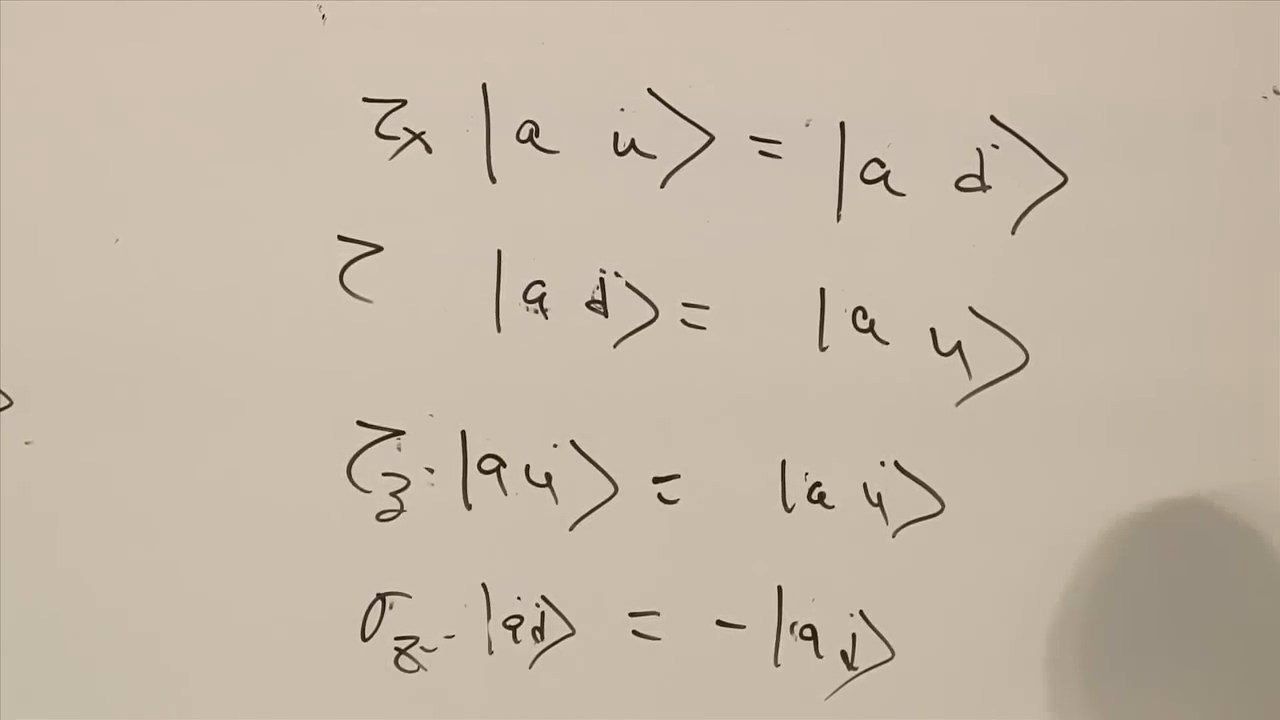
\includegraphics[width=0.86\textwidth]{lecture_06_figure_05.png}
\caption{第2スピンの作用表：第1の添字は傍観者のままである。}
\lectureframe{00:47:40}
\end{figure}

\begin{classroomqa}
\audiencequestion{\(\sigma_x\)を作用させることは、\(x\)測定が起こったことを意味するのか、そしてなぜ結果は重ね合わせにならないのか？}
\lecturerresponse{演算子の作用それ自体は測定ではない。行列\(\sigma_x\)に\(z\)基底ベクトル\(\ket{u}\)を掛けると\(\ket{d}\)が得られる。これは固有値方程式ではない。固有ベクトルなら作用の下でその向きを保つはずである。実際、\(\ket{u}\)は直交する状態に写される。これは、\(z\)固有状態に対する\(x\)測定がなぜ最大限にランダムであるかを見る別の方法である。非固有ベクトルに作用させることは、通常、計算されている完全な量から物理的意味が得られる中間的な代数的段階である。}
\end{classroomqa}

異なる因子に作用する演算子は可換である。例えば、
\begin{equation}
\sigma_x\tau_x\ket{uu}
=\ket{dd}
=\tau_x\sigma_x\ket{uu}.
\end{equation}
同じ等式がすべての合成基底ベクトルで成り立ち、したがってすべての状態で成り立つ：
\begin{equation}
[\sigma_m,\tau_n]=0
\qquad\text{for all }m,n.
\label{eq:l6-local-commutation}
\end{equation}

\begin{figure}[htbp]
\centering
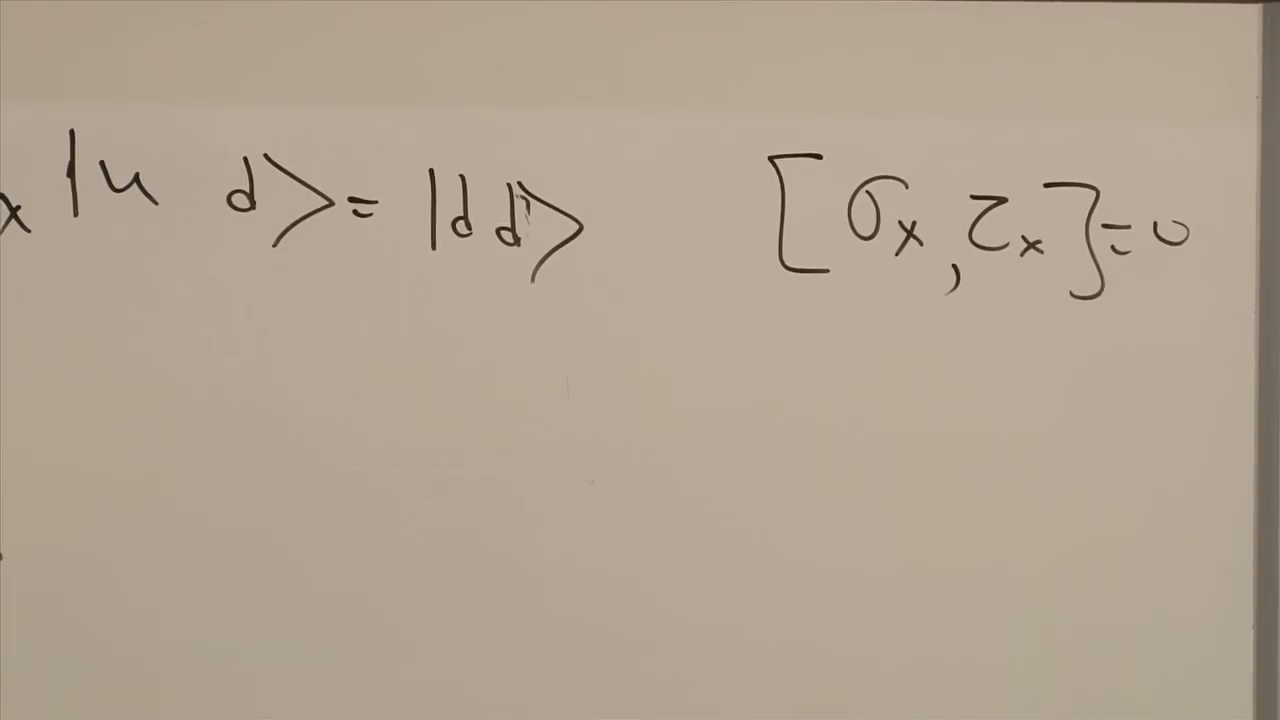
\includegraphics[width=0.86\textwidth]{lecture_06_figure_06.png}
\caption{別々のスロットへの作用は、消える交換子\([\sigma_x,\tau_x]\)を導く。}
\lectureframe{00:56:40}
\end{figure}

\begin{classroomqa}
\audiencequestion{なぜ1つの基底ベクトルを調べるだけでは、2つの演算子が可換であることの証明にならないのか？}
\lecturerresponse{演算子の等式は、すべてのベクトルへの作用が等しいことを要求する。基底のすべてのベクトルを調べれば十分である。なぜなら、線形性によって結果がすべての重ね合わせに拡張されるからである。局所演算子については、4つの基底状態すべてで議論は直ちに済む。各演算子は異なるスロットを変えるので、それらの順序は無関係である。}
\end{classroomqa}

\begin{classroomqa}
\audiencequestion{2スピン系に真に属する観測量はあるか？}
\lecturerresponse{はい。\(\sigma_x\tau_x\)、\(\sigma_x\tau_y\)のような積や、そのような積の線形結合は、結合的な性質を調べる。局所観測量は各因子を記述し、相関観測量は因子がどのように関係しているかを明らかにする。}
\end{classroomqa}

\begin{classroomqa}
\audiencequestion{独立に準備された積状態はすでにエンタングルしているか？}
\lecturerresponse{いいえ。積状態では各因子がそれ自身の状態ベクトルを持ち、局所期待値は因数分解する。エンタングルメントは、合成状態が\(\sigma\)に対する1つの状態と\(\tau\)に対する1つの状態に分離できないときに始まる。}
\end{classroomqa}

\section{一重項状態}

最大限にエンタングルした例は
\begin{equation}
\ket{S}
=\frac{1}{\sqrt2}\bigl(\ket{ud}-\ket{du}\bigr).
\label{eq:l6-singlet}
\end{equation}
である。2つの項はすでに\(z\)に沿った完全な反相関を示している。一方のスピンが上向きなら、他方は下向きである。より深い点は、どちらのスピンにもそれ自身の純粋状態を割り当てることができないということである。

\begin{figure}[htbp]
\centering
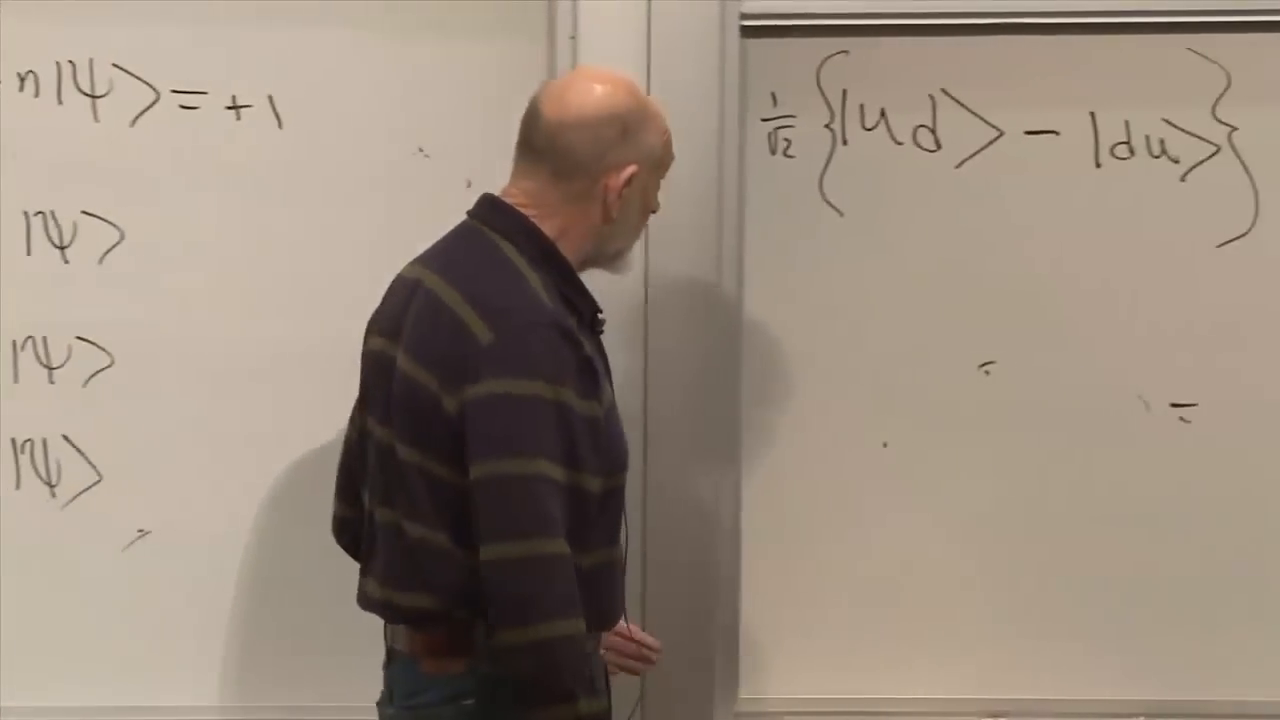
\includegraphics[width=0.86\textwidth]{lecture_06_figure_07.png}
\caption{一重項として同定される反対称な2スピン状態。}
\lectureframe{01:09:25}
\end{figure}

1スピンの純粋状態に対しては、常に単位ベクトル\(\bm n\)が存在して
\begin{equation}
(\bm\sigma\cdot\bm n)\ket{\psi}=\ket{\psi}.
\end{equation}
が成り立つ。等価に、ブロッホベクトル
\begin{equation}
\bm r
=\bigl(\expect{\sigma_x},\expect{\sigma_y},\expect{\sigma_z}\bigr)
\end{equation}
は純粋な1スピン状態に対して長さ1を持つ。したがってその3つの成分がすべて消えることはありえない。状態が与えられたとき、検出器を\(\bm r\)に沿って向けると確実に\(+1\)が得られる。おなじみの例は、\(\ket{u}\)に対する\(z\)、\((\ket{u}+\ket{d})/\sqrt2\)に対する\(x\)、そして\((\ket{u}+i\ket{d})/\sqrt2\)に対する\(y\)方向の1つである。

次に一重項における局所平均を計算する：
\begin{align}
\expect{\sigma_z}_S
&=\frac12
(\bra{ud}-\bra{du})\sigma_z
(\ket{ud}-\ket{du})\\
&=\frac12
(\bra{ud}-\bra{du})
(\ket{ud}+\ket{du})\\
&=0.
\end{align}
\(\sigma_x\)に対して、
\begin{equation}
\sigma_x\ket{S}
=\frac{\ket{dd}-\ket{uu}}{\sqrt2},
\end{equation}
これは\(\ket{S}\)に直交するので、\(\expect{\sigma_x}_S=0\)である。\(\sigma_y\)によって与えられる位相はその直交性を変えない。したがって
\begin{equation}
\expect{\sigma_x}_S
=\expect{\sigma_y}_S
=\expect{\sigma_z}_S=0.
\label{eq:l6-zero-local-sigma}
\end{equation}
対称性により、
\begin{equation}
\expect{\tau_x}_S
=\expect{\tau_y}_S
=\expect{\tau_z}_S=0.
\label{eq:l6-zero-local-tau}
\end{equation}

\begin{figure}[htbp]
\centering
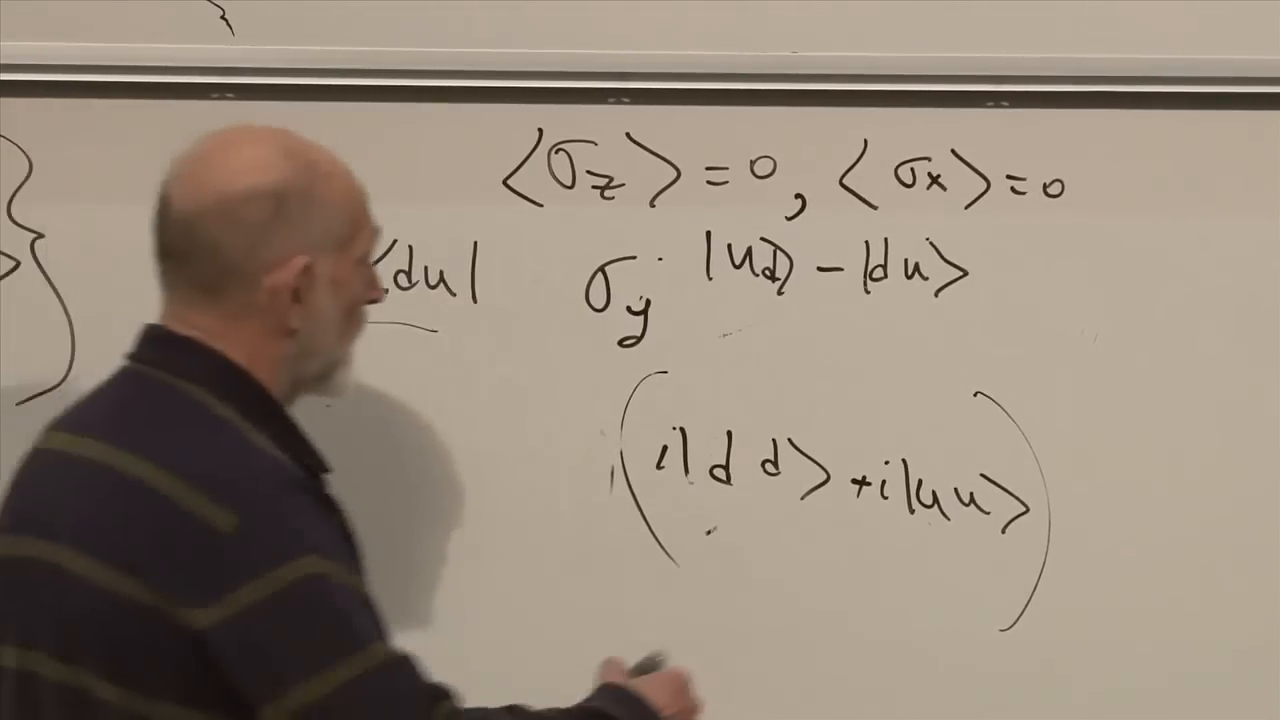
\includegraphics[width=0.86\textwidth]{lecture_06_figure_08.png}
\caption{黒板には、消える局所スピン平均と、チェックを完成させるために用いられた\(y\)成分の反転が記録されている。}
\lectureframe{01:14:20}
\end{figure}

2スピン状態全体は純粋で完全に既知であるが、各部分は局所的に偏極していない。ゼロのブロッホベクトルを持つ純粋な1スピン状態は存在しないので、\(\ket{S}\)は積状態ではありえない。

\begin{classroomqa}
\audiencequestion{通常の積状態なら、非零の局所偏極を持つ方向が依然としてあるだろうか？}
\lecturerresponse{はい。1スピンの証明は該当する因子に適用され、他方の因子は単なる傍観者である。したがって、純粋な積状態の各因子は単位ブロッホベクトルを持つ。一重項は両方のスピンについてこの積状態の性質を満たさない。}
\end{classroomqa}

\begin{classroomqa}
\audiencequestion{二つのスピンを一重項に準備するにはどうすればよいか。}
\lecturerresponse{反平行を好む結合があれば、一重項を最低エネルギー状態にできる。スピン同士を相互作用させ、その対が周囲へエネルギーを失うのを許せば、一重項へ緩和しうる。この主張は相互作用に依存する。等方的な反強磁性ハミルトニアン\(H_{\rm int}=J\,\bm\sigma\cdot\bm\tau\)（ただし\(J>0\)）では、一重項は三つの三重項状態より下に位置する。}
\end{classroomqa}

\begin{classroomqa}
\audiencequestion{その緩和にはどれだけ時間がかかるか。}
\lecturerresponse{時間スケールは、スピン間の距離、相互結合の強さ、それらの磁気モーメント、そしてエネルギーを運び去る電磁環境との結合に依存する。一般に結合が強いほど緩和は速い。}
\end{classroomqa}

\begin{classroomqa}
\audiencequestion{なぜ反対称結合の方が対称結合より低いエネルギーをもちうるのか。}
\lecturerresponse{二つのスピン\(\tfrac12\)粒子では、反対称状態は全スピン零をもち、一方、三つの対称状態は全スピン一の三重項をなす。\(+\bm\sigma\cdot\bm\tau\)に比例する相互作用は、一重項に固有値\(-3\)を、三重項に\(+1\)を割り当てるので、正の結合は一重項をより低く置く。他のハミルトニアンでは、同じように準位が順序づけられる必要はない。}
\end{classroomqa}

\subsection{どのスピン基底でも同じ状態}

より都合のよい局所基底を選んでも、もつれは取り除かれない。後に展開する基底に依存しない尺度が、もつれエントロピーである。一重項はさらに強い対称性を示す。
\begin{equation}
\ket{u}=\frac{\ket{R}+\ket{L}}{\sqrt2},
\qquad
\ket{d}=\frac{\ket{R}-\ket{L}}{\sqrt2},
\end{equation}
を式~\eqref{eq:l6-singlet}に代入すると
\begin{equation}
\ket{S}
=\frac{\ket{LR}-\ket{RL}}{\sqrt2}.
\label{eq:l6-singlet-x-basis}
\end{equation}
が得られる。任意の共通の正規直交スピン基底\(\{\ket{\rm in},\ket{\rm out}\}\)において、
\begin{equation}
\ket{S}
=\frac{\ket{{\rm in}\,{\rm out}}-\ket{{\rm out}\,{\rm in}}}{\sqrt2},
\label{eq:l6-singlet-any-basis}
\end{equation}
が、無関係な全位相を除いて成り立つ。三つの三重項状態は共通回転の下で互いに混ざり合うが、一次元の一重項部分空間はそれ自身しか再現できない。

\begin{figure}[htbp]
\centering
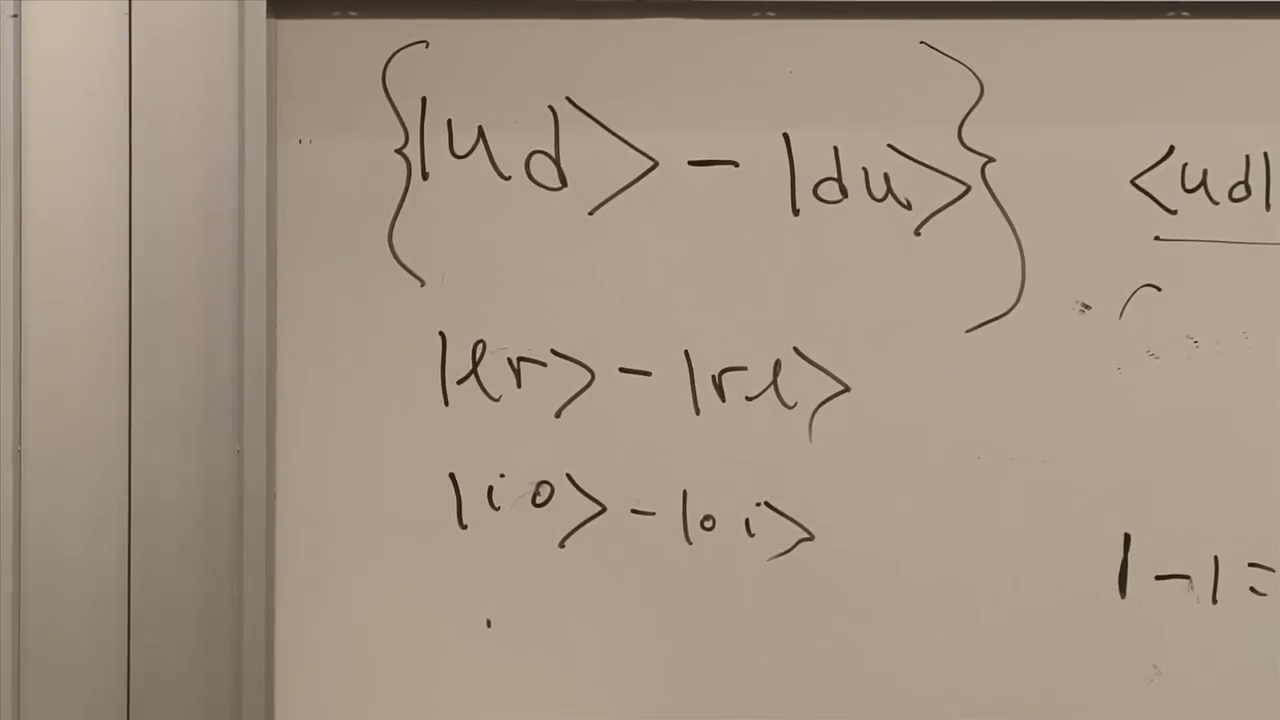
\includegraphics[width=0.86\textwidth]{lecture_06_figure_09.png}
\caption{反対称のパターンは、上-下から右-左への変更や他の共通スピン基底への変更を経ても生き残る。}
\lectureframe{01:21:00}
\end{figure}

\begin{classroomqa}
\audiencequestion{もつれは、状態を書くのに用いた基底の人為的な産物にすぎないのか。}
\lecturerresponse{否。局所基底の変更は係数を変えるが、状態が因数分解するかどうかは変えず、もつれエントロピーがその不変な事実を定量化する。一重項では、共通回転によって不変性がとりわけ可視的になる。すなわち、反対称の形はあらゆるスピン基底で再現される。}
\end{classroomqa}

\section{相関の観測量}

局所平均は消えるので、一重項の情報は結合観測量に宿らねばならない。まず
\begin{equation}
\sigma_z\tau_z\ket{ud}=-\ket{ud},
\qquad
\sigma_z\tau_z\ket{du}=-\ket{du}.
\end{equation}
から出発する。したがって
\begin{equation}
\sigma_z\tau_z\ket{S}=-\ket{S},
\qquad
\expect{\sigma_z\tau_z}_S=-1.
\label{eq:l6-zz-correlation}
\end{equation}
この結果は単なる平均ではない。一重項はその積の固有状態であり、同軸の\(z\)測定は常に反対の符号をもつ。

二つの\(x\)演算子はどちらもそのスロットを反転させる。
\begin{equation}
\sigma_x\tau_x\ket{ud}=\ket{du},
\qquad
\sigma_x\tau_x\ket{du}=\ket{ud}.
\end{equation}
二つの項を交換すると反対称状態が反転する。
\begin{equation}
\sigma_x\tau_x\ket{S}=-\ket{S},
\qquad
\expect{\sigma_x\tau_x}_S=-1.
\end{equation}
\(y\)演算子からの二つの位相は同じように相殺し、
\begin{equation}
\expect{\sigma_y\tau_y}_S=-1.
\end{equation}
を与える。対照的に、異なるデカルト成分の期待値は零である。たとえば、
\begin{equation}
\sigma_x\tau_z\ket{S}
=-\frac{\ket{dd}+\ket{uu}}{\sqrt2},
\qquad
\expect{\sigma_x\tau_z}_S=0.
\end{equation}
これらの結果はすべて
\begin{equation}
\expect{\sigma_m\tau_n}_S=-\delta_{mn},
\qquad
\expect{(\bm\sigma\cdot\bm a)(\bm\tau\cdot\bm b)}_S
=-\bm a\cdot\bm b.
\label{eq:l6-singlet-correlation-tensor}
\end{equation}
によって要約される。

\begin{figure}[htbp]
\centering
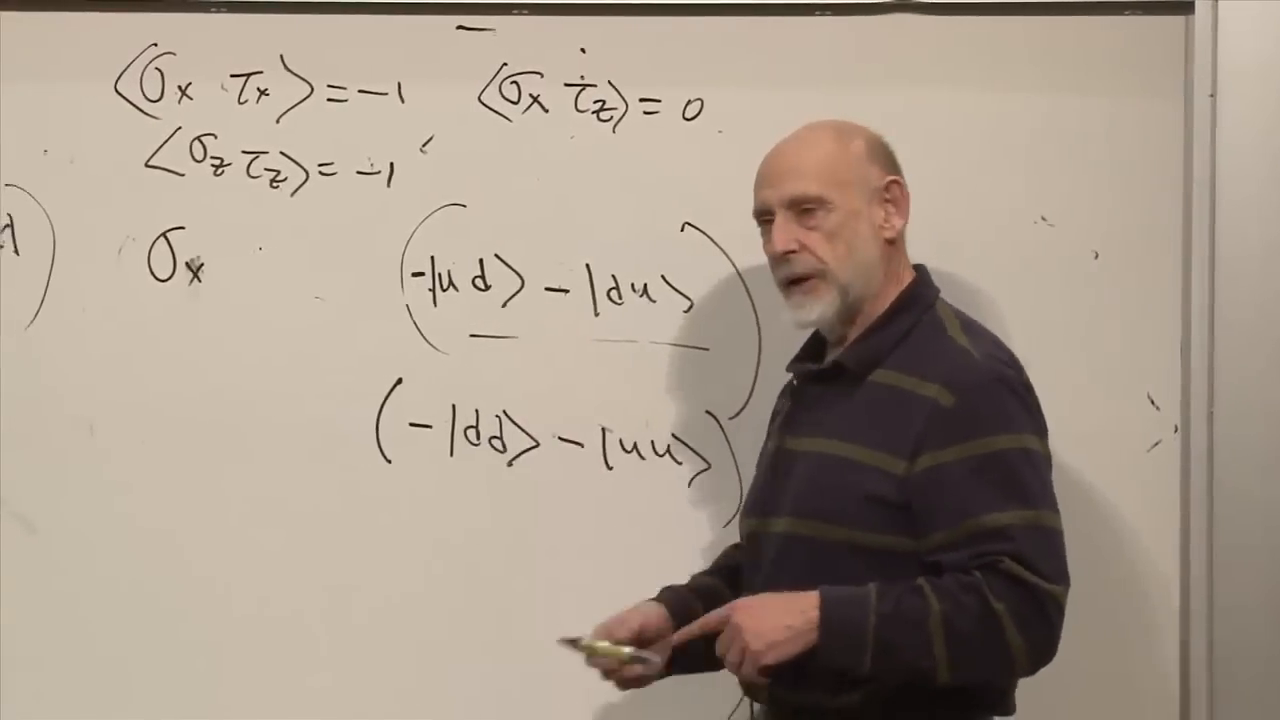
\includegraphics[width=0.86\textwidth]{lecture_06_figure_10.png}
\caption{相関の計算は\(\expect{\sigma_x\tau_x}=-1\)と混合軸の結果\(\expect{\sigma_x\tau_z}=0\)を記録している。}
\lectureframe{01:32:20}
\end{figure}

\begin{classroomqa}
\audiencequestion{二つの観測量の積は物理的に何を意味するのか。一方の測定を他方の後に行うのか。}
\lecturerresponse{一般に、エルミートな積は合成空間上の別の観測量である。ここではすべての\(\sigma_m\)がすべての\(\tau_n\)と可換なので、二つの局所成分を同時に測定し、その数値的結果を掛け合わせてよい。積演算子はその結合結果をまとめたものであり、時間順序は必要ない。}
\end{classroomqa}

積状態では、結合平均は因数分解する。
\begin{equation}
\expect{\sigma_m\tau_n}_{\rm prod}
=\expect{\sigma_m}_{\sigma}\expect{\tau_n}_{\tau}.
\end{equation}
一重項はこの因数分解を最大限に破る。右辺の各因子は零になるはずだが、左辺の同軸の積は\(-1\)である。個別にはスピンは完全にランダムであり、結合的には同じ成分は確実に反対である。

\begin{classroomqa}
\audiencequestion{二つのスピン間のあらゆる相互作用がもつれを生むのか。}
\lecturerresponse{一般的な結合は、初めに因数分解していた状態をもつれさせうるし、多くの普通の相互作用がそうする。文字どおり不可避というわけではない。特別に選ばれた積固有状態は位相だけを得るかもしれず、純粋に局所的なハミルトニアンは因子をもつれさせられない。重要なのは、それを積として保存しない状態に作用する非自明な結合である。}
\end{classroomqa}

\section{相関からベルの問いへ}

完全な反相関それ自体はパラドックスではない。小銭と10セント硬貨をポケットに入れ、見えない一方の硬貨をアリスに、他方の硬貨をボブに配り、二人を遠く離して送り出すと想像しよう。アリスは自分がどちらの硬貨を持っているかを見れば、ボブの硬貨を直ちに知る。相関は硬貨が一緒にあったときに確立されており、一方の結果を知っても他方の場所へ信号は送られない。

一重項状態はこの初等的な特徴を共有するが、決定的な自由度を加える。アリスとボブは任意の測定方向を選ぶことができ、量子力学は連続的に変化する相関\(-\bm a\cdot\bm b\)を予言する。ベルの定理は、それらすべての相関が、粒子にあらかじめ備わった局所的な古典的指示から生じうるかどうかを問う。

\begin{classroomqa}
\audiencequestion{これはベルの定理で用いられる状態ですか。}
\lecturerresponse{はい。ベル型の議論は、確定した積状態\(\ket{ud}\)ではなく、一重項状態のようなもつれ合った対を用いる。この区別は重要である。積状態は別々の局所記述を与えるのに対し、一重項状態はすべての共通基底にわたる一つの不可分な相関構造を担う。}
\end{classroomqa}

\begin{classroomqa}
\audiencequestion{等軸での結果が常に反対なら、なぜ反相関を統計的と呼ぶのですか。}
\lecturerresponse{各局所結果はランダムである。アリスは自分が\(+1\)を得るか\(-1\)を得るかを予測できない。条件付き関係は厳密である。一方の等軸結果が分かれば、他方は反対であると確定する。相関とは同時分布を指し、等軸での積における不確定性を指すのではない。}
\end{classroomqa}

この問題を鮮明にする有用な方法はシミュレーションによる。一つの古典的コンピュータは、一つのスピンに関するあらゆる実験を模倣できる。その状態を保存し、Schr\"odinger方程式で時間発展させ、要求された確率を計算し、乱数生成器を用いて結果を選ぶ。繰り返し測定も磁気歳差もすべて再現できる。

次に、もつれ合った対を二つの古典的コンピュータに分けよう。対が準備されている間はコンピュータ同士が相互作用することを許し、その後で接続を切り、遠く離れた場所で測定方向を独立に選ぶ。あらかじめ固定された共有乱数を持っていても、分離した局所古典プログラムの対は、方向のあらゆる選択に対して量子相関を再現できない。大域的な古典シミュレーションは可能だが、それは結合状態へのアクセスを保持するか、局所隠れ変数模型ではない仕方で両側を調整しなければならない。

この局所古典的記帳の失敗は、光速を超える通信路を与えるものではない。アリスの局所結果は依然としてランダムであり、したがって彼女は、ボブが後に記録を比較せずに読めるメッセージを制御できない。非局所性をめぐる用語はさまざまだが、操作上の区別は固い。ベル相関は局所古典的説明を排除しつつ、ノーシグナリングを保つ。

したがって、複合状態の構成は真に新しいものを生み出した。テンソル積は古い一スピンの物理を局所的に保つが、その一般的なベクトルは別々の状態に分割できない。一重項状態では、すべての局所偏極が消える一方、結合スピン成分は完全で基底に依存しない反相関を担う。次の段階は、この構造を古典的推論に対するベルの定量的検証へと変えることである。
